\apendice{Documentación Técnica de Programación}
\label{apendice:doc_tecnica}


\section{Introducción}
Este anexo está dirigido a un perfil técnico (un futuro desarrollador o evaluador del proyecto) y tiene como objetivo detallar la estructura del código, la arquitectura de los componentes de software, las decisiones de diseño y el proceso completo de compilación y despliegue del sistema. La finalidad es que cualquier persona con los conocimientos técnicos adecuados pueda comprender, replicar y extender el trabajo realizado.

\section{Estructura de Directorios del Repositorio}
\label{sec:doc_tecnica_directorios}
La organización del repositorio en GitHub ha sido una pieza clave para mantener el proyecto ordenado y comprensible. A continuación, se expone la estructura de directorios que cuelgan desde la raíz del proyecto.

\subsection{Directorio de Documentación (`/docs`)}
La carpeta \texttt{/docs} contiene toda la documentación del proyecto, principalmente la memoria del TFG y sus recursos asociados. Su estructura es la siguiente:

\dirtree{%
.1 /docs.
.2 /diagrams.
.2 /images.
.2 /tex.
.2 memoria.tex.
.2 anexos.tex.
.2 bibliografia.bib.
}

\begin{itemize}
    \item \texttt{/diagrams}: Almacena los ficheros fuente de los diagramas del proyecto (por ejemplo, los archivos de \textit{Diagrams.net}).
    \item \texttt{/images} (o \texttt{/img}): Contiene los ficheros de imagen (PNG, JPG) que se insertan en la memoria, como capturas de pantalla o los diagramas exportados.
    \item \texttt{/tex}: Contiene los ficheros \texttt{.tex} individuales para cada capítulo y apéndice de la memoria, permitiendo una organización modular del documento.
    \item \texttt{memoria.tex} y \texttt{anexos.tex}: Son los ficheros principales de \LaTeX{} que estructuran y compilan el documento final.
    \item \texttt{bibliografia.bib}: Fichero de BibTeX que contiene todas las referencias bibliográficas citadas.
\end{itemize}

\subsection{Directorio de Configuración del Despliegue}
Esta carpeta contiene los ficheros de configuración validados y necesarios para desplegar los sistemas de terceros, principalmente Jitsi. No contiene una instancia de Jitsi, sino las plantillas para configurarla a partir del repositorio oficial.

\dirtree{%
.1 /configuracion\_despliegue.
.2 /jitsi.
.3 .gitkeep.
.3 README.md.
.3 docker-compose.yml.
.3 env.example.
.3 gen-passwords.sh.
.3 jibri.yml.
}
Un desarrollador que desee replicar el entorno debe clonar el repositorio oficial de \texttt{docker-jitsi-meet} y utilizar los ficheros de esta carpeta como base para su configuración.

\subsection{Directorio de Código Fuente (`/src`)}
La carpeta \texttt{/src} es el corazón del proyecto. Contiene todo el código fuente de la aplicación de procesamiento y su fichero de orquestación con Docker Compose.

\dirtree{%
.1 /src.
.2 /data.
.3 /processed.
.4 .gitkeep.
.3 .gitkeep.
.2 /dockers.
.3 /python\_processor.
.4 main.py.
.4 requirements.txt.
.4 Dockerfile.
.2 docker-compose.yml.
}

\begin{itemize}
    \item \texttt{docker-compose.yml}: Es el fichero de orquestación que define y levanta los servicios del pipeline de procesamiento de datos: Kafka, Spark (master y worker) y el procesador Python.
    \item \texttt{/dockers/python\_processor}: Contiene la lógica de la aplicación principal.
        \begin{itemize}
            \item \texttt{Dockerfile}: Instrucciones para construir la imagen Docker del servicio.
            \item \texttt{requirements.txt}: Lista de las librerías de Python necesarias para el proyecto.
            \item \texttt{main.py}: El script principal que contiene la lógica para detectar, procesar y archivar los vídeos.
        \end{itemize}
    \item \texttt{/data}: Actúa como punto de montaje principal para los datos de vídeo. Los vídeos grabados por Jibri se mapean a este directorio para que el pipeline los pueda procesar. Contiene a su vez las subcarpetas \texttt{/processed} y \texttt{/archived} para almacenar los resultados y los ficheros originales, respectivamente.
\end{itemize}

\section{Manual del Programador (Arquitectura del Software)}

\subsection{Arquitectura Modular}
El sistema se ha diseñado siguiendo un enfoque modular, separando claramente dos responsabilidades principales:
\begin{itemize}
    \item \textbf{Sistema de Captura (Jitsi):} Se encarga exclusivamente de la captura y grabación de las sesiones de vídeo, generando los archivos MP4.
    \item \textbf{Pipeline de Procesamiento (Kafka/Spark):} Es un sistema independiente que se encarga de consumir y procesar dichos archivos.
\end{itemize}
Esta separación facilita el desarrollo, las pruebas y la escalabilidad, ya que cada componente puede ser modificado o sustituido sin afectar al otro.

\subsection{Arquitectura del Pipeline de Procesamiento}
La Figura \ref{fig:flujo_pipeline} (incluida en el Apéndice de Diseño) ilustra la interacción entre los servicios definidos en el fichero \texttt{docker-compose.yml} de la carpeta \texttt{/src}.
\begin{itemize}
    \item \textbf{Kafka:} Actúa como \textit{broker} de mensajería para desacoplar el sistema. Funciona en modo KRaft, sin dependencia de Zookeeper.
    \item \textbf{Spark (Master/Worker):} Conforman el clúster de cómputo donde se ejecutan las tareas de procesamiento de vídeo.
    \item \textbf{python-processor:} Es el servicio principal que contiene la lógica de negocio. Orquesta todo el flujo: detecta los vídeos, los envía a Kafka, y consume los resultados de Spark.
\end{itemize}

\begin{figure}[H]
    \centering
    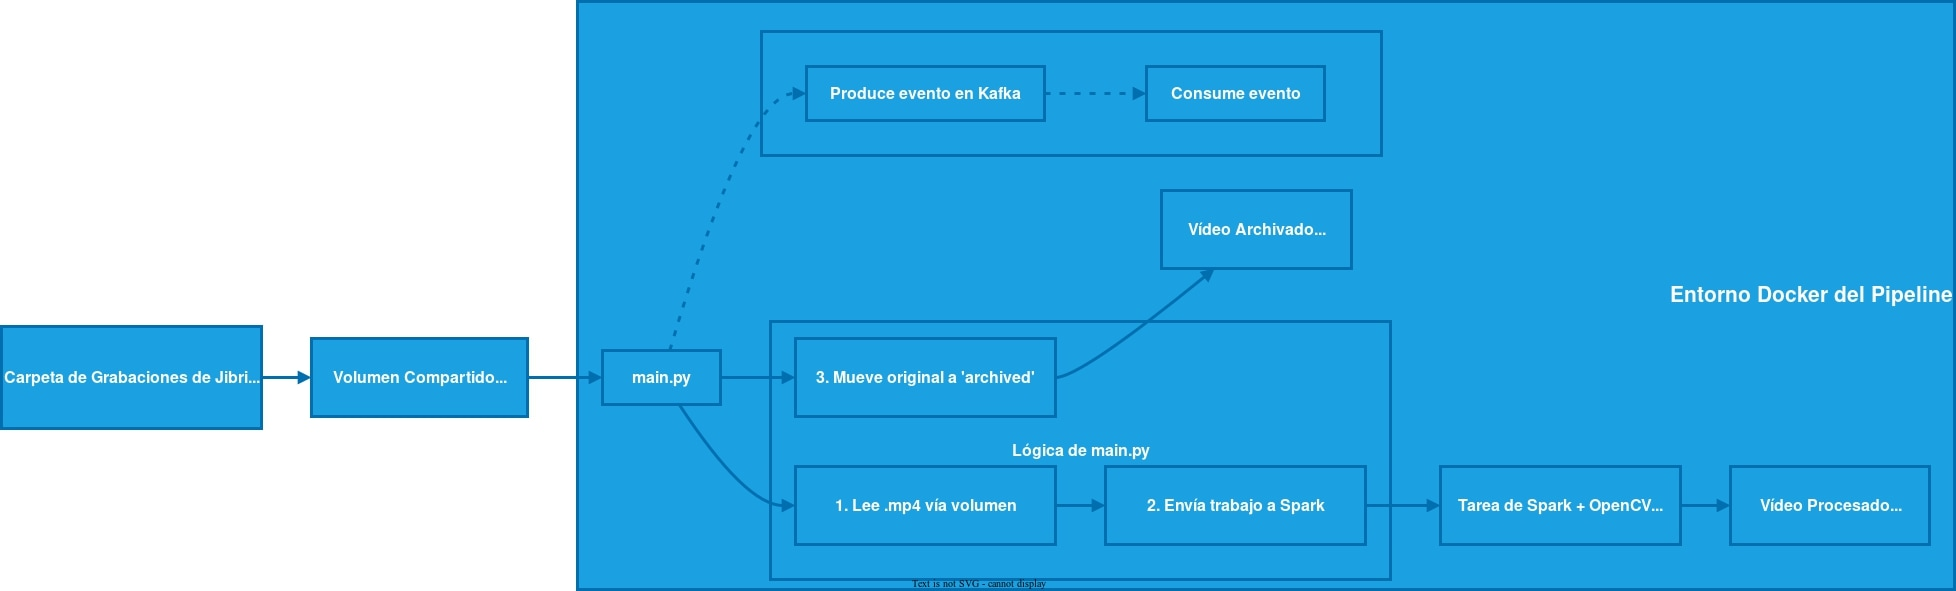
\includegraphics[width=\textwidth]{img/FlujodeDatosdelPipelinedeProcesamiento.jpg}
    \caption{Diagrama de flujo de datos del pipeline de procesamiento implementado en la carpeta /src.}
    \label{fig:apendice_d_flujo_pipeline}
\end{figure}

\subsection{Descripción del Script \texttt{main.py}}
El script \texttt{main.py} es el cerebro de la aplicación. Su lógica principal es la siguiente:
\begin{enumerate}
    \item Establece una conexión con la sesión de Spark para poder enviar trabajos de procesamiento.
    \item Entra en un bucle que busca el vídeo más antiguo en la carpeta de entrada (\texttt{/data}), ignorando explícitamente los subdirectorios \texttt{/processed} y \texttt{/archived}.
    \item Si encuentra un vídeo, lo envía a un \textit{topic} de Kafka y espera el resultado del procesamiento.
    \item Una vez procesado, guarda el vídeo resultante y archiva el original.
\end{enumerate}

\begin{figure}[H]
    \centering
    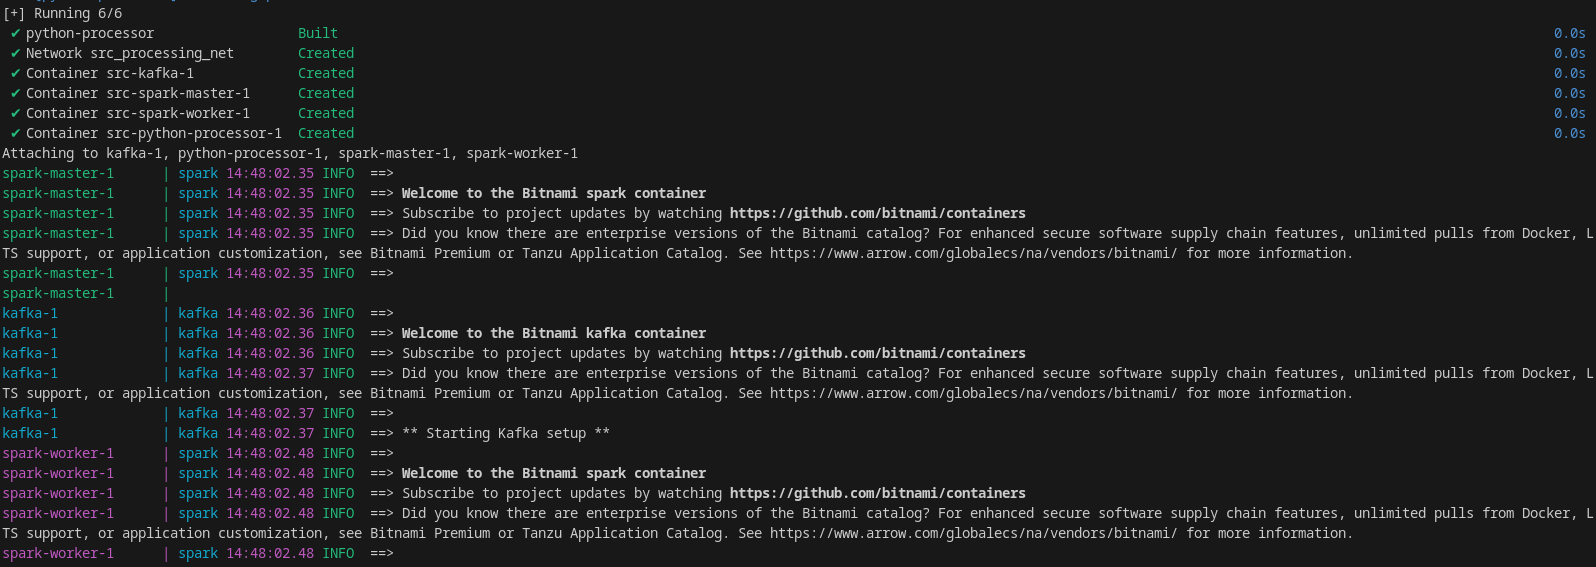
\includegraphics[width=\textwidth]{img/montarsparkkafka.png}
    \caption{Salida de la terminal mostrando el despliegue de los servicios del pipeline (Kafka, Spark, etc.) con Docker Compose.}
    \label{fig:apendice_d_compose_up}
\end{figure}

\subsection{Construcción de la Imagen Docker (Dockerfile)}
El \texttt{Dockerfile} del servicio \texttt{python-processor} define los pasos para construir su imagen. Las decisiones clave fueron:
\begin{itemize}
    \item Usar una imagen base oficial de Python (\texttt{python:3.9-slim}) por ser ligera y estable.
    \item Instalar las dependencias de sistema necesarias, como Java, que es un requisito para la comunicación con Spark.
    \item Instalar las librerías de Python especificadas en el fichero \texttt{requirements.txt}, \\ fijando las versiones para garantizar la reproducibilidad y evitar conflictos (como el surgido con NumPy).
\end{itemize}

\section{Compilación, Instalación y Ejecución del Proyecto}

\subsection{Configuración del Entorno Anfitrión}
Los requisitos detallados del sistema anfitrión se encuentran en el Apéndice E. Los puntos clave son el uso de Debian como sistema operativo, la instalación de Docker y Docker Compose, y la instalación del módulo del kernel \texttt{v4l2loopback-dkms} para el correcto funcionamiento de Jibri.

\subsection{La Crónica del Despliegue de Jitsi}
El despliegue de Jitsi fue uno de los mayores desafíos de ingeniería de este proyecto. El proceso de depuración se puede resumir en los siguientes hitos:
\begin{enumerate}
    \item \textbf{Fracaso en Windows/WSL2:} El intento inicial de despliegue en este entorno falló debido a problemas insuperables de permisos de ficheros y autenticación de los servicios.
    \item \textbf{Pivote a Debian:} Se tomó la decisión estratégica de migrar a un entorno Linux nativo, lo que solucionó los problemas de base.
    \item \textbf{Depuración de la Conexión:} Se resolvieron sucesivamente problemas de conexión WSS, errores de montaje del fichero \texttt{custom.config.js} y fallos de autenticación de usuarios invitados en Prosody.
    \item \textbf{Implementación de HTTPS:} Se descartó el uso de certificados autofirmados por problemas de confianza y se implementó una solución robusta con \textbf{Let's Encrypt}, para lo cual fue necesario configurar un dominio público con DuckDNS y re-dirección de puertos.
    \item \textbf{Diagnóstico del "Vídeo en Negro":} El problema final de la falta de vídeo en las grabaciones de Jibri se diagnosticó como una necesidad de permisos elevados, solucionándose al añadir la directiva \texttt{privileged: true} al servicio.
\end{enumerate}

\begin{figure}[H]
    \centering
    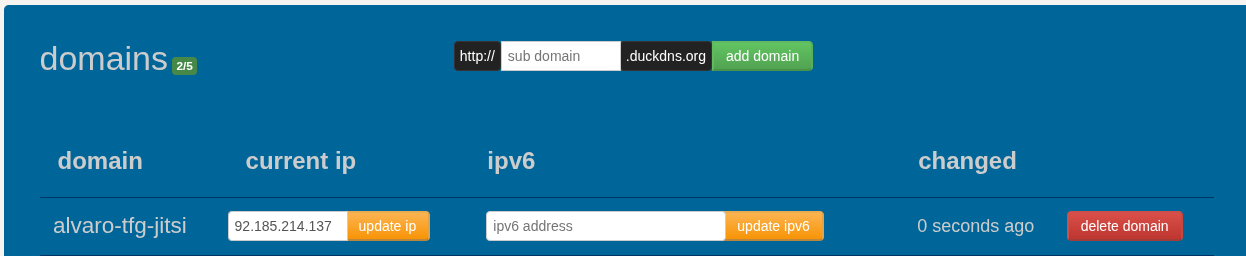
\includegraphics[width=0.9\textwidth]{img/duckdns.png}
    \caption{Configuración del dominio público en el servicio de DNS Dinámico DuckDNS.}
    \label{fig:apendice_d_duckdns}
\end{figure}

\begin{figure}[H]
    \centering
    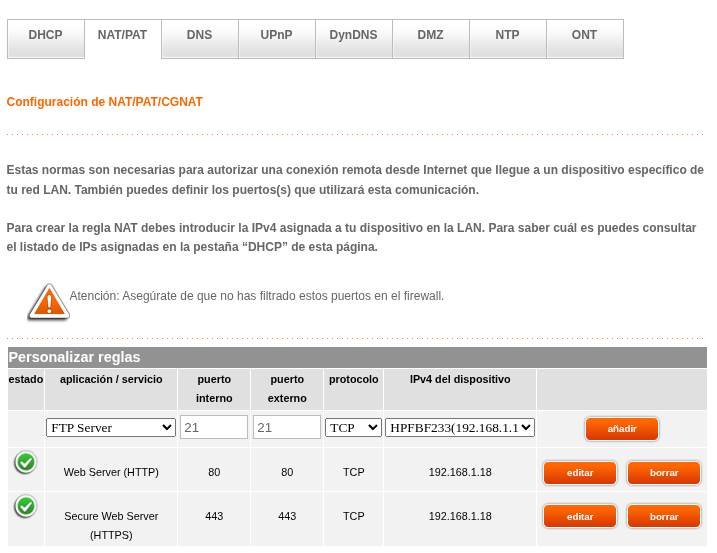
\includegraphics[width=0.9\textwidth]{img/routerconfig.png}
    \caption{Configuración de la redirección de puertos en el router para permitir el acceso externo a Jitsi.}
    \label{fig:apendice_d_router}
\end{figure}

\begin{figure}[H]
    \centering
    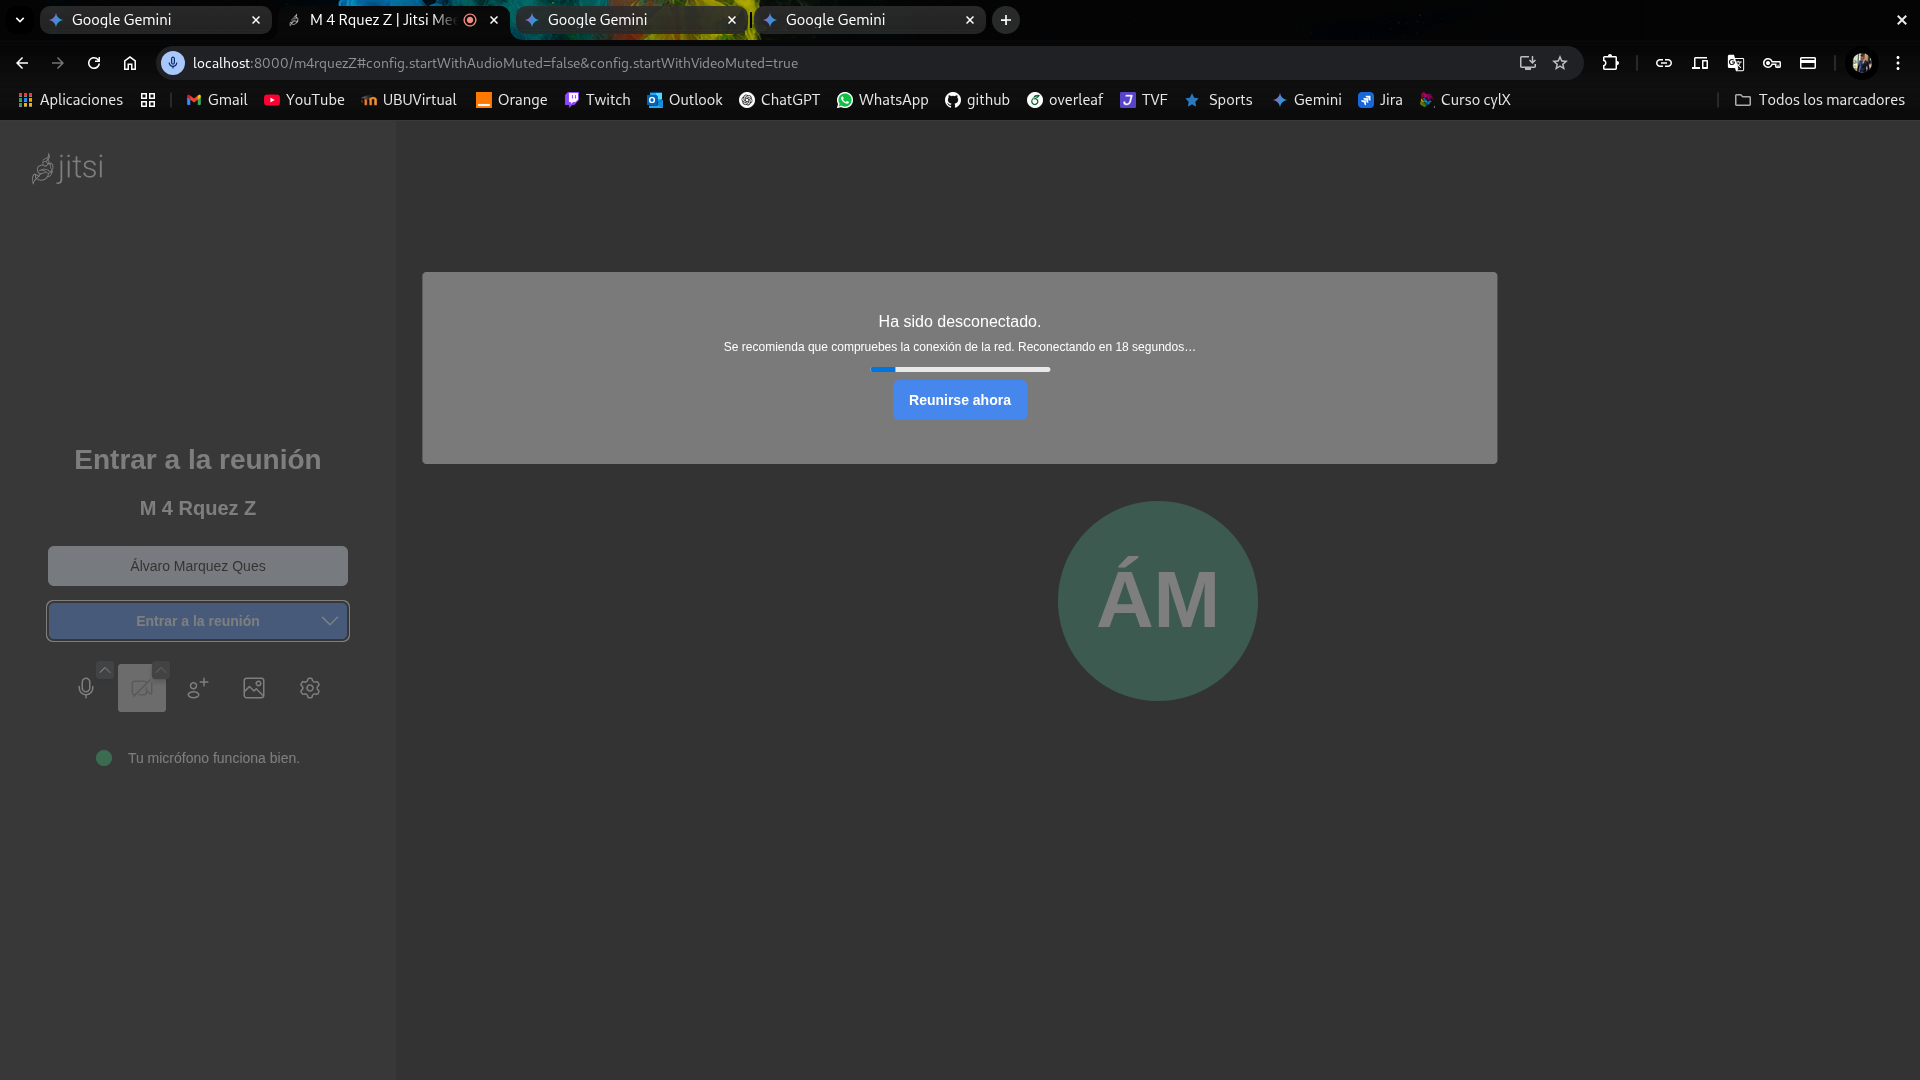
\includegraphics[width=0.7\textwidth]{img/errorconexion.png}
    \caption{Error de conexión encontrado durante la depuración de Jitsi en Debian.}
    \label{fig:apendice_d_error_conexion}
\end{figure}

\subsection{Despliegue del Pipeline de Procesamiento}
El despliegue de la pila de Kafka y Spark es un proceso automatizado. Al ejecutar \texttt{docker compose up} en el directorio \texttt{/src}, todos los servicios se inician en el orden correcto. La conexión con Jitsi se realiza a través del volumen Docker compartido que mapea la carpeta de grabaciones de Jibri al directorio de entrada del pipeline.

\begin{figure}[H]
    \centering
    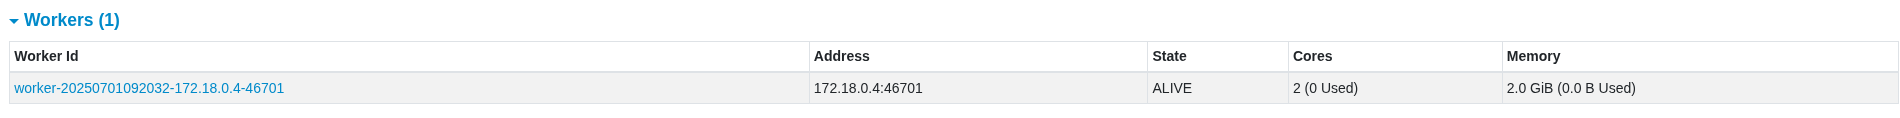
\includegraphics[width=0.9\textwidth]{img/workerpy.png}
    \caption{Captura de servicio \textit{worker} levantado y corriendo.}
    \label{fig:worker_py}
\end{figure}

\section{Pruebas del Sistema}

\subsection{Pruebas de Integración}
Se ha probado el flujo completo de extremo a extremo:
\begin{enumerate}
    \item Se inicia una conferencia en Jitsi y se graba.
    \item Se verifica que Jibri genera y guarda correctamente el archivo MP4.
    \item Se ejecuta el pipeline de procesamiento.
    \item Se comprueba en los \textit{logs} que el \textit{script} detecta el vídeo, lo procesa y lo archiva.
    \item Se verifica la existencia y el contenido del vídeo procesado en la carpeta de salida.
\end{enumerate}
Estas pruebas han validado que todos los componentes se comunican correctamente entre sí.

\subsection{Pruebas Funcionales (Prueba de Concepto)}
Para demostrar la funcionalidad del procesamiento, se ha implementado un algoritmo simple que invierte los colores de cada fotograma. La Figura \ref{fig:prueba_funcional} muestra una comparación entre un fotograma del vídeo original y el mismo fotograma del vídeo procesado, donde se puede apreciar visualmente el éxito de la transformación aplicada.

\begin{figure}[H]
    \centering
    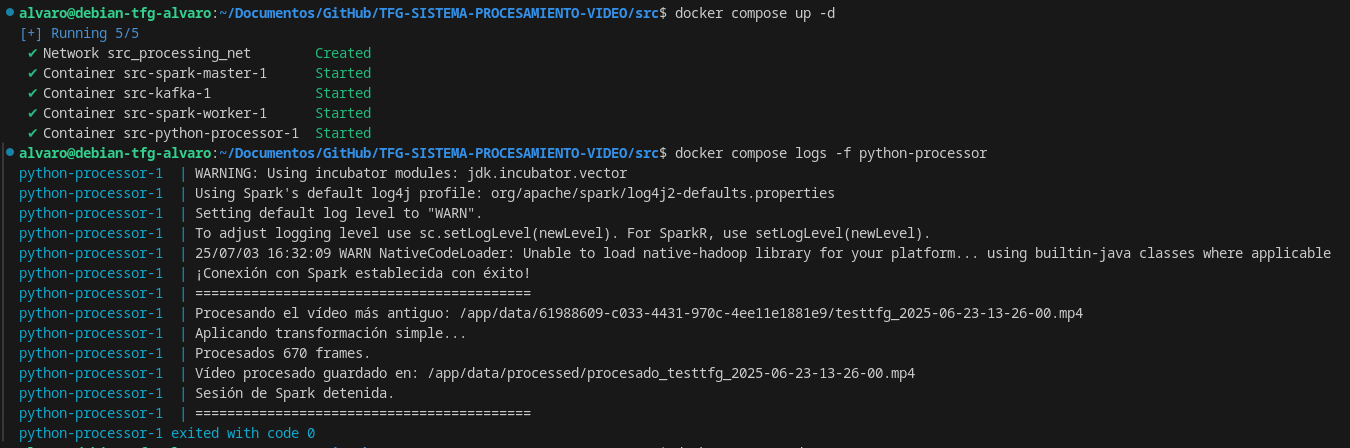
\includegraphics[width=\textwidth]{img/logsfinalpy.png}
    \caption{Logs del contenedor \texttt{python-processor} que muestran la ejecución exitosa del pipeline completo.}
    \label{fig:apendice_d_logs_finales}
\end{figure}
\begin{figure}[H]
    \centering
    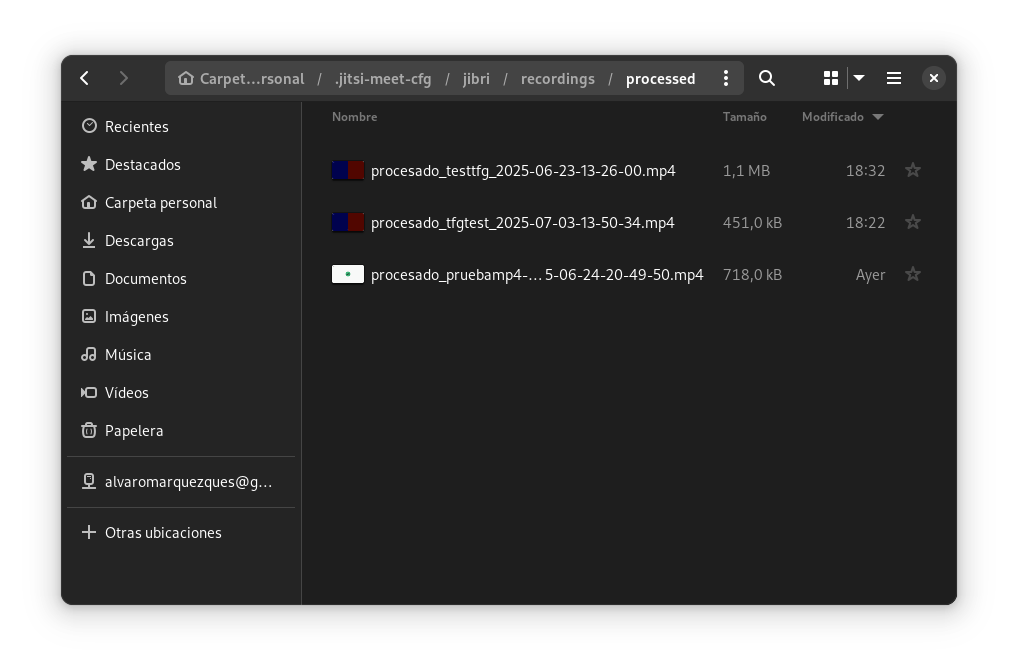
\includegraphics[width=1\textwidth]{img/carpetaprocessed.png}
    \caption{Directorio de salida con el fichero de vídeo ya procesado.}
    \label{fig:apendice_d_carpeta_procesado}
\end{figure}
\begin{figure}[H]
    \centering
    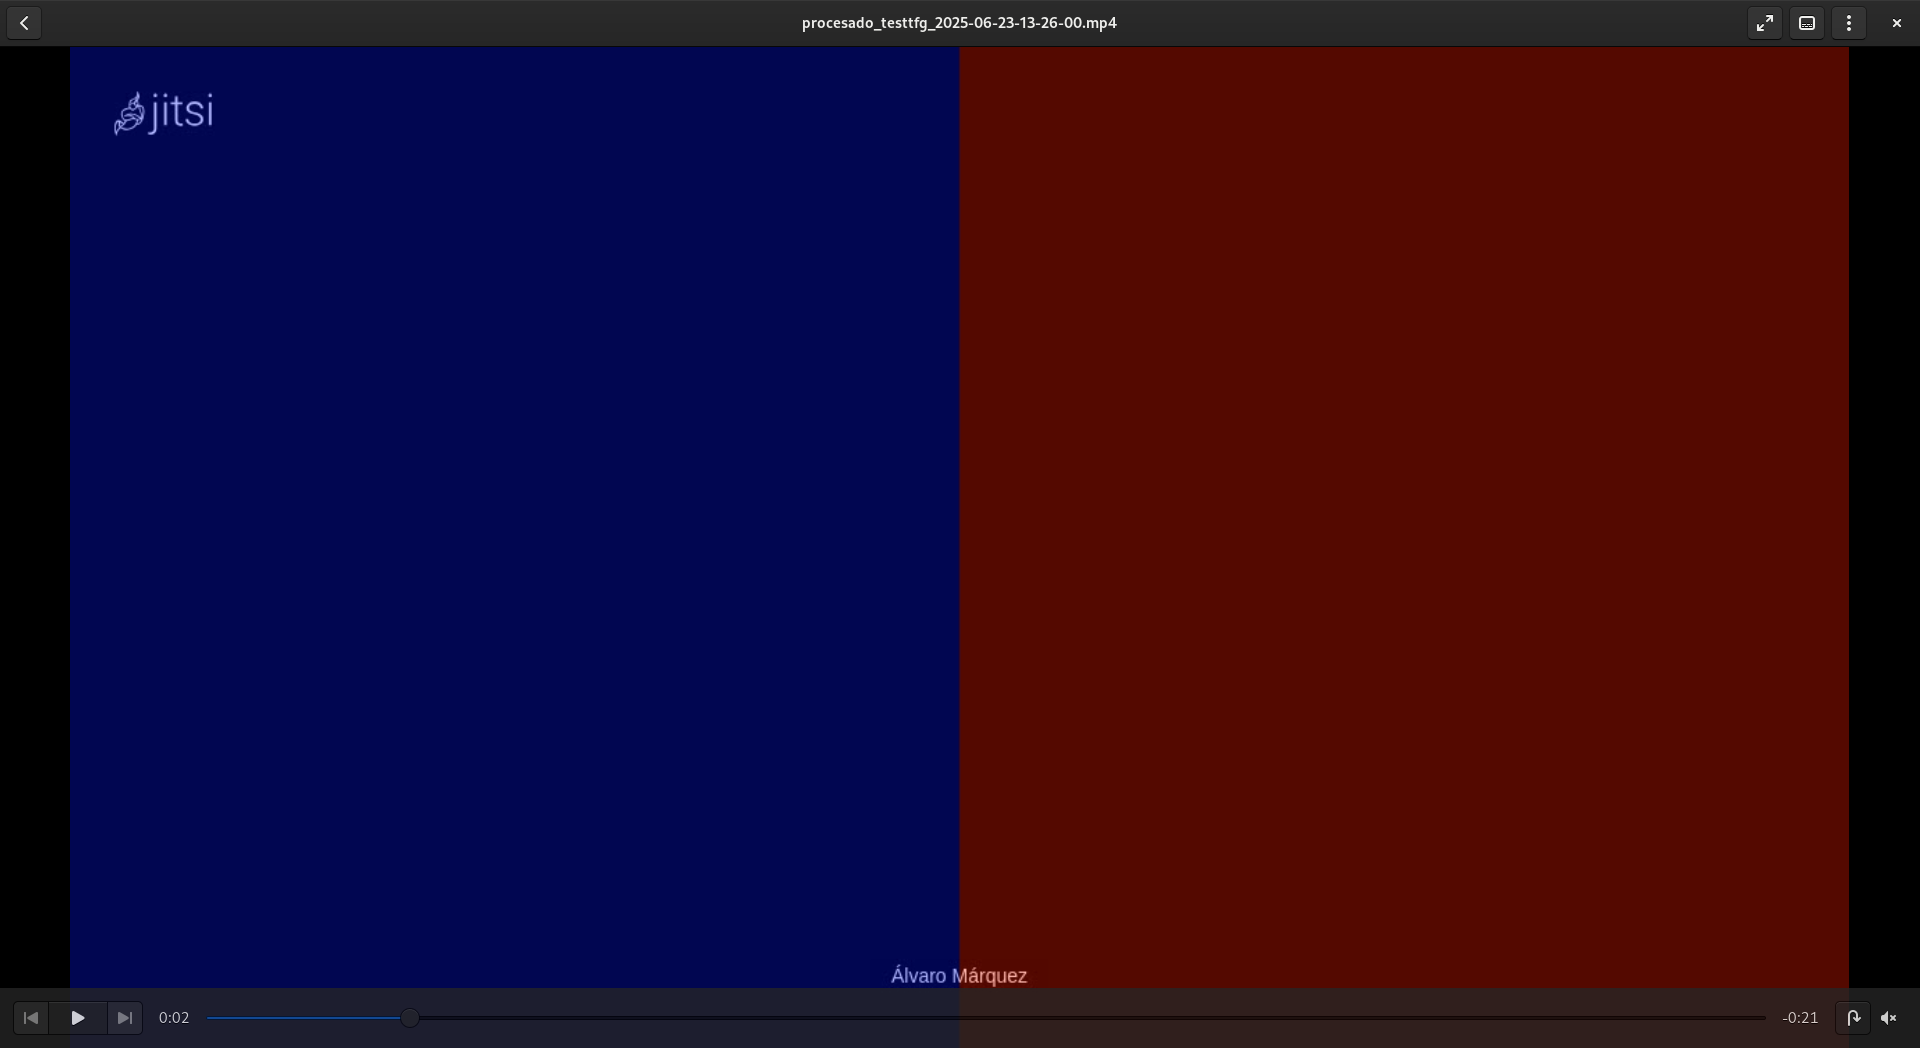
\includegraphics[width=0.9\textwidth]{img/resultado-procesamiento.png}
    \caption{Captura de video ya procesado.}
    \label{fig:prueba_funcional}
\end{figure}

\section{Fallos y Soluciones}
\label{sec:fallos_soluciones}
En este apartado se exponen algunos de los errores y desafíos técnicos más relevantes por los que se ha visto comprometido el proyecto a lo largo de su desarrollo. Se detalla para cada uno el síntoma observado, el diagnóstico técnico de la causa raíz y la solución final que se implementó.

\subsection{Fallo 1: Inestabilidad Crítica del Despliegue en Entorno Windows (WSL2)}
\begin{itemize}
    \item \textbf{Síntoma:} Inoperabilidad total de la pila \texttt{docker-jitsi-meet}. El \textit{log} del contenedor Prosody (servidor de autenticación) mostraba errores críticos y repetitivos de \texttt{Permission denied}. El contenedor Jibri no lograba arrancar o entraba en un bucle de reinicios, mostrando en sus logs errores de autenticación \texttt{SASLError}.
    
    \item \textbf{Diagnóstico Técnico:} Se determinó que existía un conflicto irresoluble en la traducción de permisos entre el sistema de ficheros de Windows (NTFS) y el de Linux (ext4) que usan los contenedores. La capa de virtualización de WSL2 no gestionaba adecuadamente los permisos de propietario/grupo (\texttt{chown}/\texttt{chgrp}) que los servicios de Jitsi necesitaban para operar.
    
    \item \textbf{Solución Aplicada:} Abandono completo del entorno Windows. Se realizó una instalación nativa de Debian 12, proporcionando un entorno de sistema de ficheros y permisos 100\% compatible, lo que se considera la solución estándar para despliegues de servidor robustos.
\end{itemize}

\subsection{Fallo 2: Despliegue de Jitsi en Debian - Errores de Conexión en Cascada}
\begin{itemize}
    \item \textbf{Síntoma:} Tras un despliegue exitoso en Debian, la interfaz web no permitía unirse a una sala, mostrando el error "La conexión ha fallado". La depuración reveló múltiples problemas encadenados: el cliente web intentaba una conexión segura (WSS) en un servidor HTTP, un posterior error de montaje \texttt{not a directory} al intentar forzar la configuración con \texttt{custom.config.js}, y finalmente un error de "Ha sido desconectado" al entrar en una sala.
    
    \item \textbf{Diagnóstico Técnico:} Se diagnosticaron tres problemas independientes: 1) una configuración por defecto del cliente que forzaba WSS; 2) la creación accidental de un directorio en lugar de un fichero de configuración en el \textit{host}; y 3) la falta de un \texttt{VirtualHost} en la configuración de Prosody para la autenticación de usuarios invitados.
    
    \item \textbf{Solución Aplicada:} Se solucionó cada problema de forma secuencial: se creó correctamente el fichero \texttt{custom.config.js} para forzar la conexión HTTP y, crucialmente, se modificó el fichero de configuración \texttt{jitsi-meet.cfg.lua} de Prosody para añadir la configuración del \texttt{VirtualHost} de invitados.
\end{itemize}

\begin{figure}[H]
    \centering
    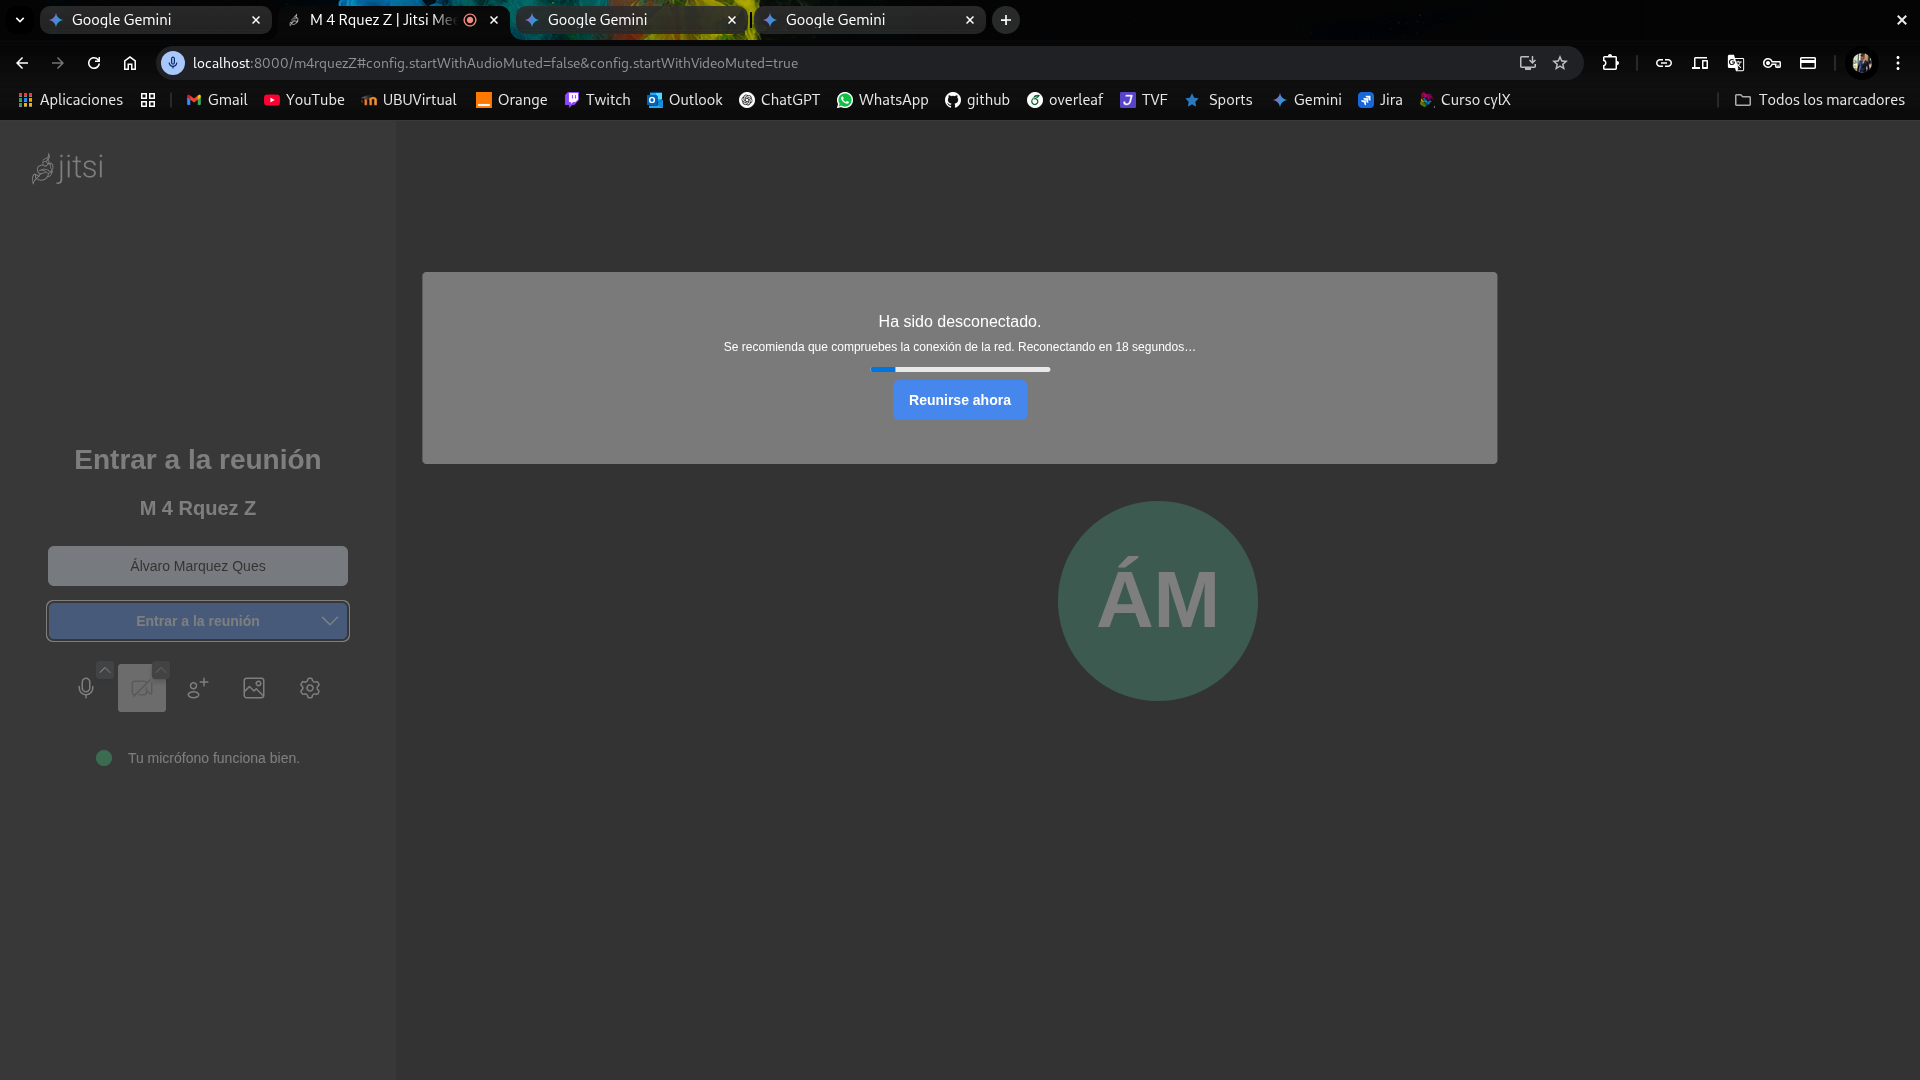
\includegraphics[width=0.9\textwidth]{img/errorconexion.png}
    \caption{Capture de error persistente de Conexión.}
    \label{fig:anexod_error_conexion}
\end{figure}

\subsection{Fallo 3: Problemas de Red para la Validación de Certificados SSL}
\begin{itemize}
    \item \textbf{Síntoma:} Al intentar implementar HTTPS con Let's Encrypt, el proceso de validación de certificados fallaba.
    \item \textbf{Diagnóstico Técnico:} Se determinó que los servidores de Let's Encrypt no podían alcanzar la máquina anfitriona en los puertos 80 y 443. Esto se debía a la naturaleza dinámica de la IP doméstica y a la falta de configuración en el \textit{router} local.
    \item \textbf{Solución Aplicada:} Se implementó una configuración de red completa: 1) Se configuró un DNS dinámico con \textbf{DuckDNS}. 2) Se asignó una IP local estática a la máquina Debian mediante reserva de DHCP en el router. 3) Se configuró la re-dirección de puertos (\textit{Port Forwarding}) en el \textit{router} para dirigir el tráfico de los puertos 80 y 443 a la IP fija de la máquina Debian.
\end{itemize}

\subsection{Fallo 4: Grabaciones de Jibri con Vídeo en Negro}
\begin{itemize}
    \item \textbf{Síntoma:} El servicio Jibri generaba un fichero \texttt{.mp4} del tamaño correcto, pero este estaba completamente en negro y sin sonido.
    \item \textbf{Diagnóstico Técnico:} El análisis de los \textit{logs} de Jibri (\texttt{(EE) no screens found(EE)}) reveló que el entorno gráfico virtual (Xvfb) no podía iniciarse. La causa raíz fue la falta del módulo del kernel \texttt{v4l2loopback} en el sistema anfitrión Debian, necesario para crear un dispositivo de vídeo virtual del cual grabar.
    \item \textbf{Solución Aplicada:} Se realizó la instalación del módulo requerido en el \textit{host} con el comando \texttt{sudo apt install v4l2loopback-dkms} y se reinició el sistema.
\end{itemize}

\subsection{Fallo 5: Errores Durante la Construcción de una Imagen Docker Personalizada}
\begin{itemize}
    \item \textbf{Síntoma:} Al intentar construir una imagen de Jibri personalizada para depurar, el proceso \texttt{docker build} fallaba con errores de \texttt{apt-get update}.
    \item \textbf{Diagnóstico Técnico:} Se identificaron dos problemas en el \texttt{Dockerfile} base: 1) una clave GPG expirada de un repositorio de Google Chrome y 2) la referencia a un paquete obsoleto (\texttt{libindicator3-7}).
    \item \textbf{Solución Aplicada:} Se modificó el \texttt{Dockerfile} para eliminar el fichero de repositorio problemático antes de ejecutar \texttt{apt-get update} y se reemplazó el paquete obsoleto por su sucesor, \\ \texttt{libayatana-appindicator3-1}.
\end{itemize}

\subsection{Fallo 6: Conflictos y Errores en el Pipeline de Spark}
\begin{itemize}
    \item \textbf{Síntoma:} Al levantar el pipeline de procesamiento, surgieron múltiples errores: un conflicto de puertos (8080), errores de importación en Python (`ModuleNotFoundError`, `numpy.core.multiarray failed to import`), una excepción `java.io.InvalidClassException`, una "condición de carrera" al conectar con Spark y un bucle de procesamiento infinito.
    \item \textbf{Diagnóstico Técnico:} Se diagnosticaron cinco problemas distintos: 1) Conflicto del puerto del Spark Master con el Jitsi Videobridge. 2) Falta de un fichero \texttt{requirements.txt} y un conflicto de versiones entre OpenCV y NumPy. 3) Incompatibilidad entre la versión de la librería PySpark y la imagen Docker de Spark. 4) El \textit{script} de Python intentaba conectar antes de que el máster de Spark estuviera listo. 5) El \textit{script} no tenía lógica para gestionar los vídeos ya procesados.
    \item \textbf{Solución Aplicada:} Se aplicaron soluciones específicas para cada problema: 1) Se cambió el puerto del Spark Master al 8081. 2) Se creó un \texttt{requirements.txt} fijando las versiones (\texttt{pyspark==3.5.0}, \texttt{numpy<2.0}). 3) Se fijó la versión de la imagen de Spark a \\(\texttt{bitnami/spark:3.5.0}. 4) Se añadió un retardo de 10 segundos \\ (\texttt{time.sleep(10)}) al inicio del \textit{script}. 5) Se implementó la lógica de mover el vídeo original a una carpeta \texttt{/archived} tras su procesamiento.
\end{itemize}